%%%%%%%%%%%%%%%%%%%%%%%%%%%%%%%%%%%%%%%%%%%%%%
% Head matter - can we try to be consistent on
% included packages
\documentclass{beamer}
\mode<presentation>
{\usetheme{default}
 \usecolortheme{default}
 \usefonttheme{default}
 \setbeamertemplate{navigation symbols}{}
 \setbeamertemplate{footline}[frame number]
% \setbeamertemplate{caption}[numbered]
 }
\usepackage[english]{babel}
\usepackage{algorithm}
\usepackage[noend]{algpseudocode}
\usepackage[utf8x]{inputenc}
\usepackage{graphicx}
\usepackage{hyperref}
%\graphicspath{{./images/}}
\usepackage{tikz}
\usetikzlibrary{shapes.geometric, arrows,chains}
\usepackage{booktabs,makecell,multirow,tabularx}
\usepackage{verbatim}
\renewcommand{\arraystretch}{1.2}
\renewcommand\theadfont{\normalfont\bfseries}
\usepackage{array}
\usepackage{eqnarray,amsmath}
\usepackage{listings}
\lstset{language=Java, showstringspaces=false}
\usepackage[normalem]{ulem}
\usepackage{bm}
\def\layersep{2.5cm}

\usepackage{xcolor}
%\usepackage{subfig}
\setbeamertemplate{caption}{\insertcaption}
\usepackage[caption=false]{subfig}
\usepackage{hyperref}
\usepackage{verbatim}
%\setbeamertemplate{caption}[numbered]%\numberwithin{figure}{section}
% Define block styles
\tikzstyle{decision} = [diamond, draw, fill=blue!20, 
    text width=4.5em, text badly centered, node distance=3cm, inner sep=0pt]
\tikzstyle{block} = [rectangle, draw, fill=blue!20, 
    text width=3em, text centered, rounded corners, minimum height=3em]
\tikzstyle{line} = [draw, -latex']
\tikzstyle{cloud} = [draw, ellipse, fill=red!20, node distance=3cm,
    minimum height=2em]
\tikzset{
  startstop/.style={
    rectangle, 
    rounded corners,
    minimum width=3cm, 
    minimum height=1cm,
    align=center, 
    draw=black, 
    fill=red!30
    },
  process/.style={
    rectangle, 
    minimum width=3cm, 
    minimum height=1cm, 
    align=center, 
    draw=black, 
    fill=blue!30
    },
  decision/.style={
    rectangle, 
    minimum width=3cm, 
    minimum height=1cm, align=center, 
    draw=black, 
    fill=green!30
    },
  arrow/.style={thick,->,>=stealth},
  dec/.style={
    ellipse, 
    align=center, 
    draw=black, 
    fill=green!30
    },
}
\tikzstyle{arrow} = [thick,->,>=stealth]

\tikzset{onslide/.code args={<#1>#2}{%
  \only<#1>{\pgfkeysalso{#2}} % \pgfkeysalso doesn't change the path
}}

\makeatletter
\newenvironment<>{btHighlight}[1][]
{\begin{onlyenv}#2\begingroup\tikzset{bt@Highlight@par/.style={#1}}\begin{lrbox}{\@tempboxa}}
{\end{lrbox}\bt@HL@box[bt@Highlight@par]{\@tempboxa}\endgroup\end{onlyenv}}

\newcommand<>\btHL[1][]{%
  \only#2{\begin{btHighlight}[#1]\bgroup\aftergroup\bt@HL@endenv}%
}
\def\bt@HL@endenv{%
  \end{btHighlight}%   
  \egroup
}
\newcommand{\bt@HL@box}[2][]{%
  \tikz[#1]{%
    \pgfpathrectangle{\pgfpoint{1pt}{0pt}}{\pgfpoint{\wd #2}{\ht #2}}%
    \pgfusepath{use as bounding box}%
    \node[anchor=base west, fill=orange!30,outer sep=0pt,inner xsep=1pt, inner ysep=0pt, rounded corners=3pt, minimum height=\ht\strutbox+1pt,#1]{\raisebox{1pt}{\strut}\strut\usebox{#2}};
  }%
}
\makeatother




%%%%%%%%%%%%%%%%%%%%%%%%%%%%%%%%%%%%%%%%%%%%%%
% Formatting for title page
\title[Deep Learning]{Variational Autoencoders}
\author{Kate Farrahi}
\institute{ECS Southampton}
\date{\today}
%%%%%%%%%%%%%%%%%%%%%%%%%%%%%%%%%%%%%%%%%%%%%%
\begin{document}
\begin{frame}
  \titlepage
\end{frame}
%-------------------------------------------------------------%

%\begin{frame}[fragile]{pause}\frametitle{Vanishing Gradients in RNNs}
%\end{frame}
%-------------------------------------------------------------%

\begin{frame}[fragile]{pause}\frametitle{Variational Autoencoder (VAE)}
	\begin{itemize}
		\item VAEs architecturally similar to autoencoders (AEs). 
		\item VAEs (vs AEs) significantly different in their goal and mathematical formulation.
		\item AEs map the input into a fixed vector. 
		\item However, VAEs map the input into a distribution. 
		\item VAEs are a combination of neural networks (AEs) and \bf{graphical models}.
	\end{itemize}
\end{frame}
%-------------------------------------------------------------%

\begin{frame}[fragile]{pause}\frametitle{Graphical Models (Background)}
	\begin{itemize}
		\item A graphical model is a probabilistic model for which a graph expresses the conditional dependence structure between random variables. 
		\item Graphical models are commonly used in probability theory, statistics —particularly Bayesian statistics— and machine learning. \footnote{Definition taken from Wikipedia}
	\end{itemize}
\end{frame}

%-------------------------------------------------------------%

\begin{frame}[fragile]{pause}\frametitle{KL Divergence (Background)}
	\begin{itemize}
		\item Kullback–Leibler divergence, $D_{\text{KL}}(P\parallel Q)$: a measure of how one probability distribution $Q$ is different from a second, reference probability distribution $P$. \footnote{Definition taken from Wikipedia}
		\item A simple interpretation of the divergence of P from Q is the expected excess surprise from using Q as a model when the actual distribution is P. 
		\item While it is a distance, it is not a metric, the most familiar type of distance: it is asymmetric in the two distributions.
	\end{itemize}
\end{frame}
%-------------------------------------------------------------%

\begin{frame}[fragile]\frametitle{Variational Autoencoders (VAEs)}
	
%\begin{center}
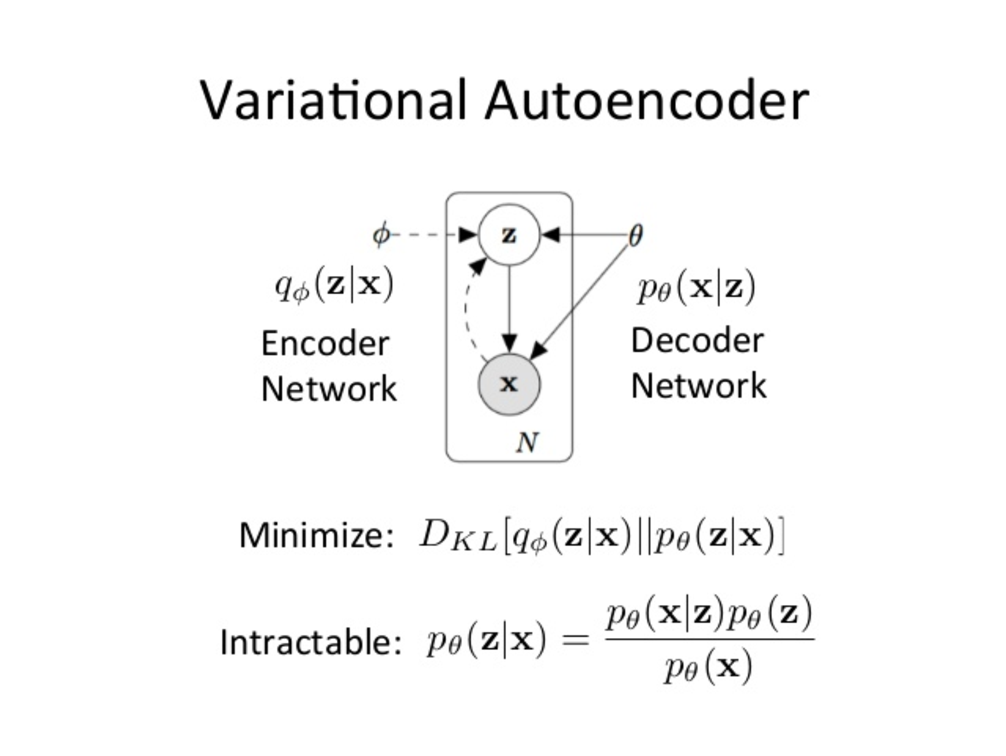
\includegraphics[width=10cm]{VAE.pdf} \footnote{Auto-Encoding Variational Bayes \url{https://arxiv.org/abs/1312.6114}}
%\end{center}
\end{frame}


%-------------------------------------------------------------%


\begin{frame}[fragile]\frametitle{Variational Autoencoders (VAEs)}
	\begin{center}
	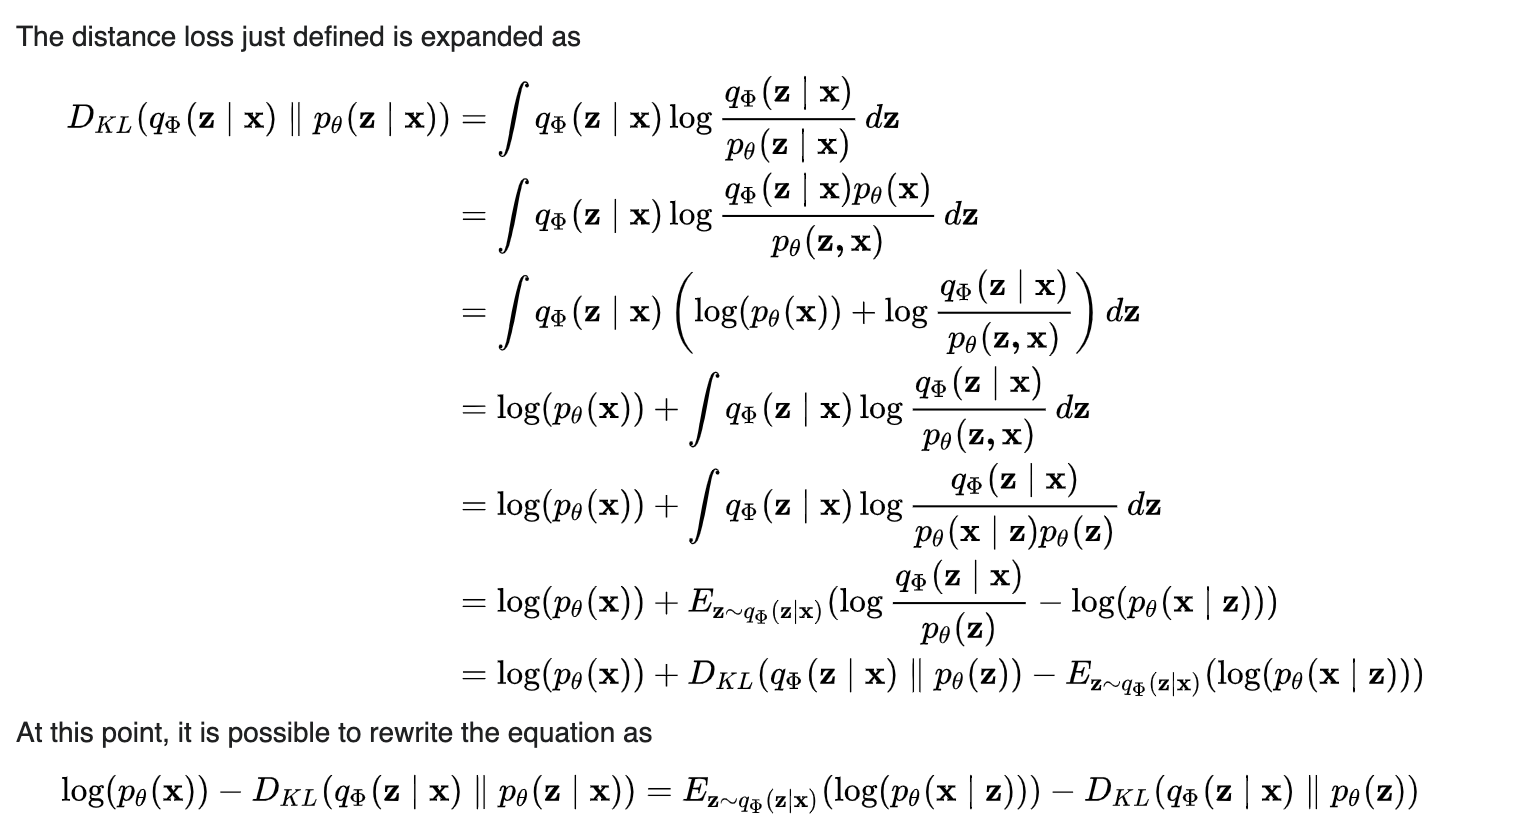
\includegraphics[width=10cm]{VAE_formulation.png}
	\end{center}
\end{frame}

%-------------------------------------------------------------%



\begin{frame}[fragile]\frametitle{ Evidence Lower Bound (ELBO) Loss}
	\begin{equation*}
	L_{VAE}(\theta, \phi) = - \mathbb{E}_{z\sim q_{\phi}(z|x)} log (p_{\theta}(x|z)) +  D_{KL}(q_{\phi}(z|x)|| p_{\theta}(z))
	\end{equation*}

\begin{itemize}
	\item We are trying to minimize the ELBO loss with respect to the model parameters.
\end{itemize}
\end{frame}


%%-------------------------------------------------------------%


\begin{frame}[fragile]\frametitle{Why Autoencoder?}
	
		\begin{itemize}
		\item The reconstruction term, forces each image to be unique and spread out.
		
		\item The KL term will push all the images towards the same prior.
		
		\end{itemize}

	\begin{center}
		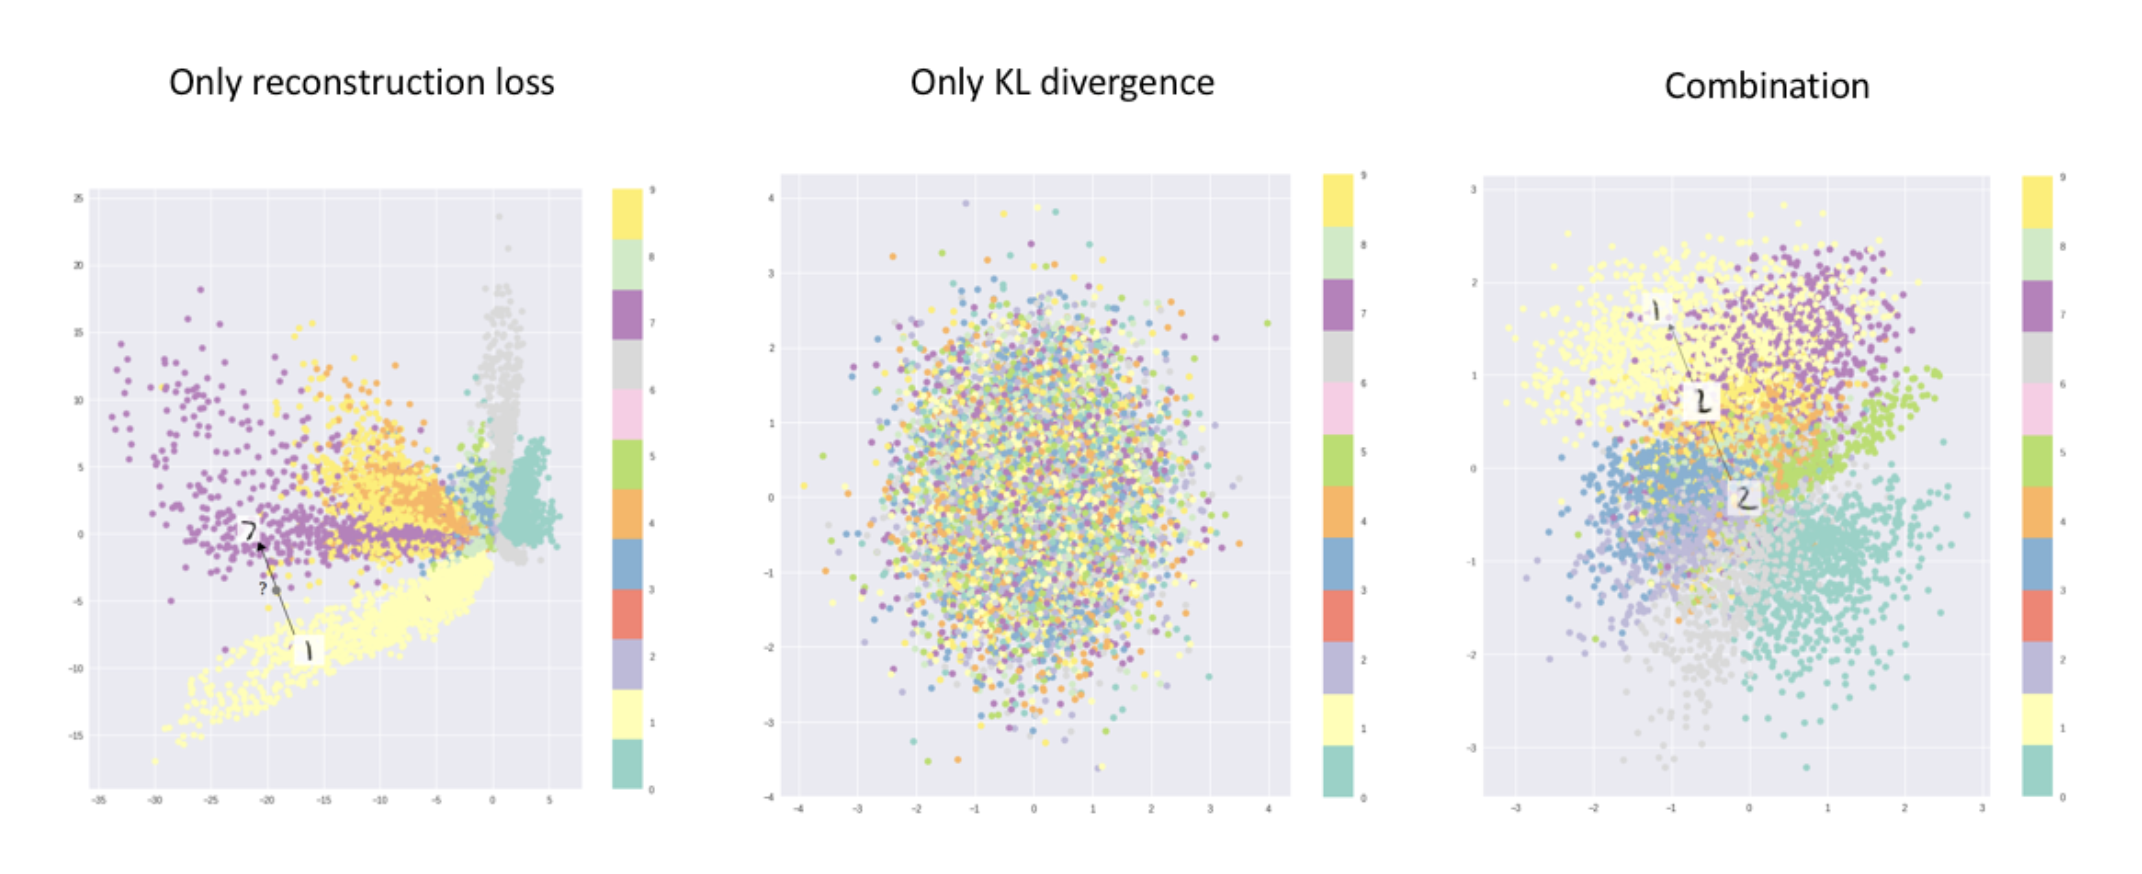
\includegraphics[width=10cm]{loss_vis.png} \footnote{Figure taken from https://towardsdatascience.com/intuitively-understanding-variational-autoencoders-1bfe67eb5daf}
	\end{center}
\end{frame}

%-------------------------------------------------------------%

%\begin{frame}[fragile]\frametitle{Why Autoencoder?}
%	\begin{center}
%		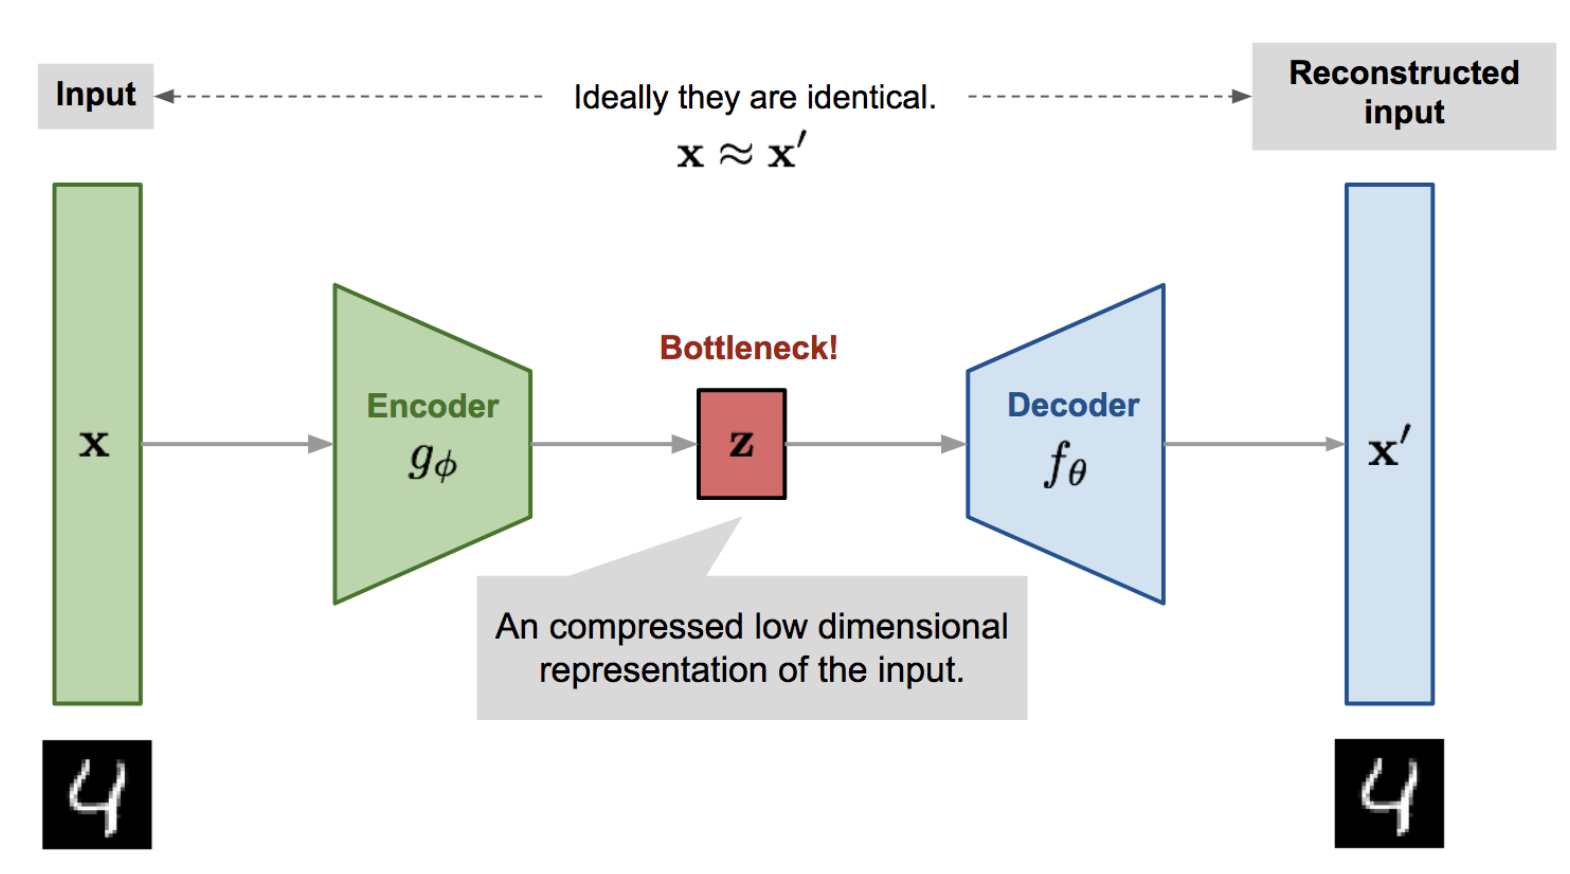
\includegraphics[width=10cm]{samplingprocess.png}
%	\end{center}
%\end{frame}

%-------------------------------------------------------------%

%
%\begin{frame}[fragile]\frametitle{Why is it called an Autoencoder?}
%	\begin{itemize}
%		\item $q(z|x)$ is referred to as an encoder; it's used to take $x$ and turn it into a $z$. \pause
%		\item $p(x^{'}|z)$ is a decoder network; it takes a $z$ and decodes it into a target $x^{'}$.
%		\item From a practical standpoint, a VAE is a normal AE with two key differences
%		\begin{enumerate}
%			\item the encoder generates a distribution that must be sampled
%			\item the decoder generates a distribution, not a sample. 
%		\end{enumerate}
%	\end{itemize}
%\end{frame}

%-------------------------------------------------------------%


\begin{frame}[fragile]\frametitle{Training Procedure}
	\begin{center}
		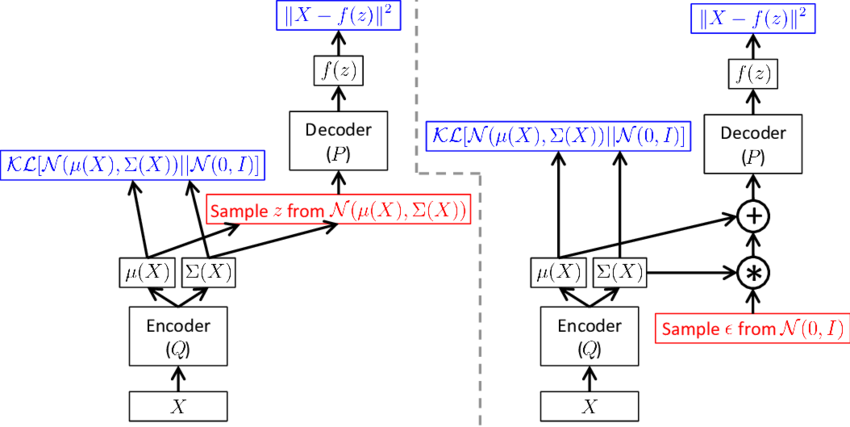
\includegraphics[width=10cm]{train_VAE.png} \footnote{Figure taken from Carl Doersch tutorial}
	\end{center}
\end{frame}

%-------------------------------------------------------------%

\begin{frame}[fragile]\frametitle{Reparametrization Trick Visualisation}
	\begin{center}
		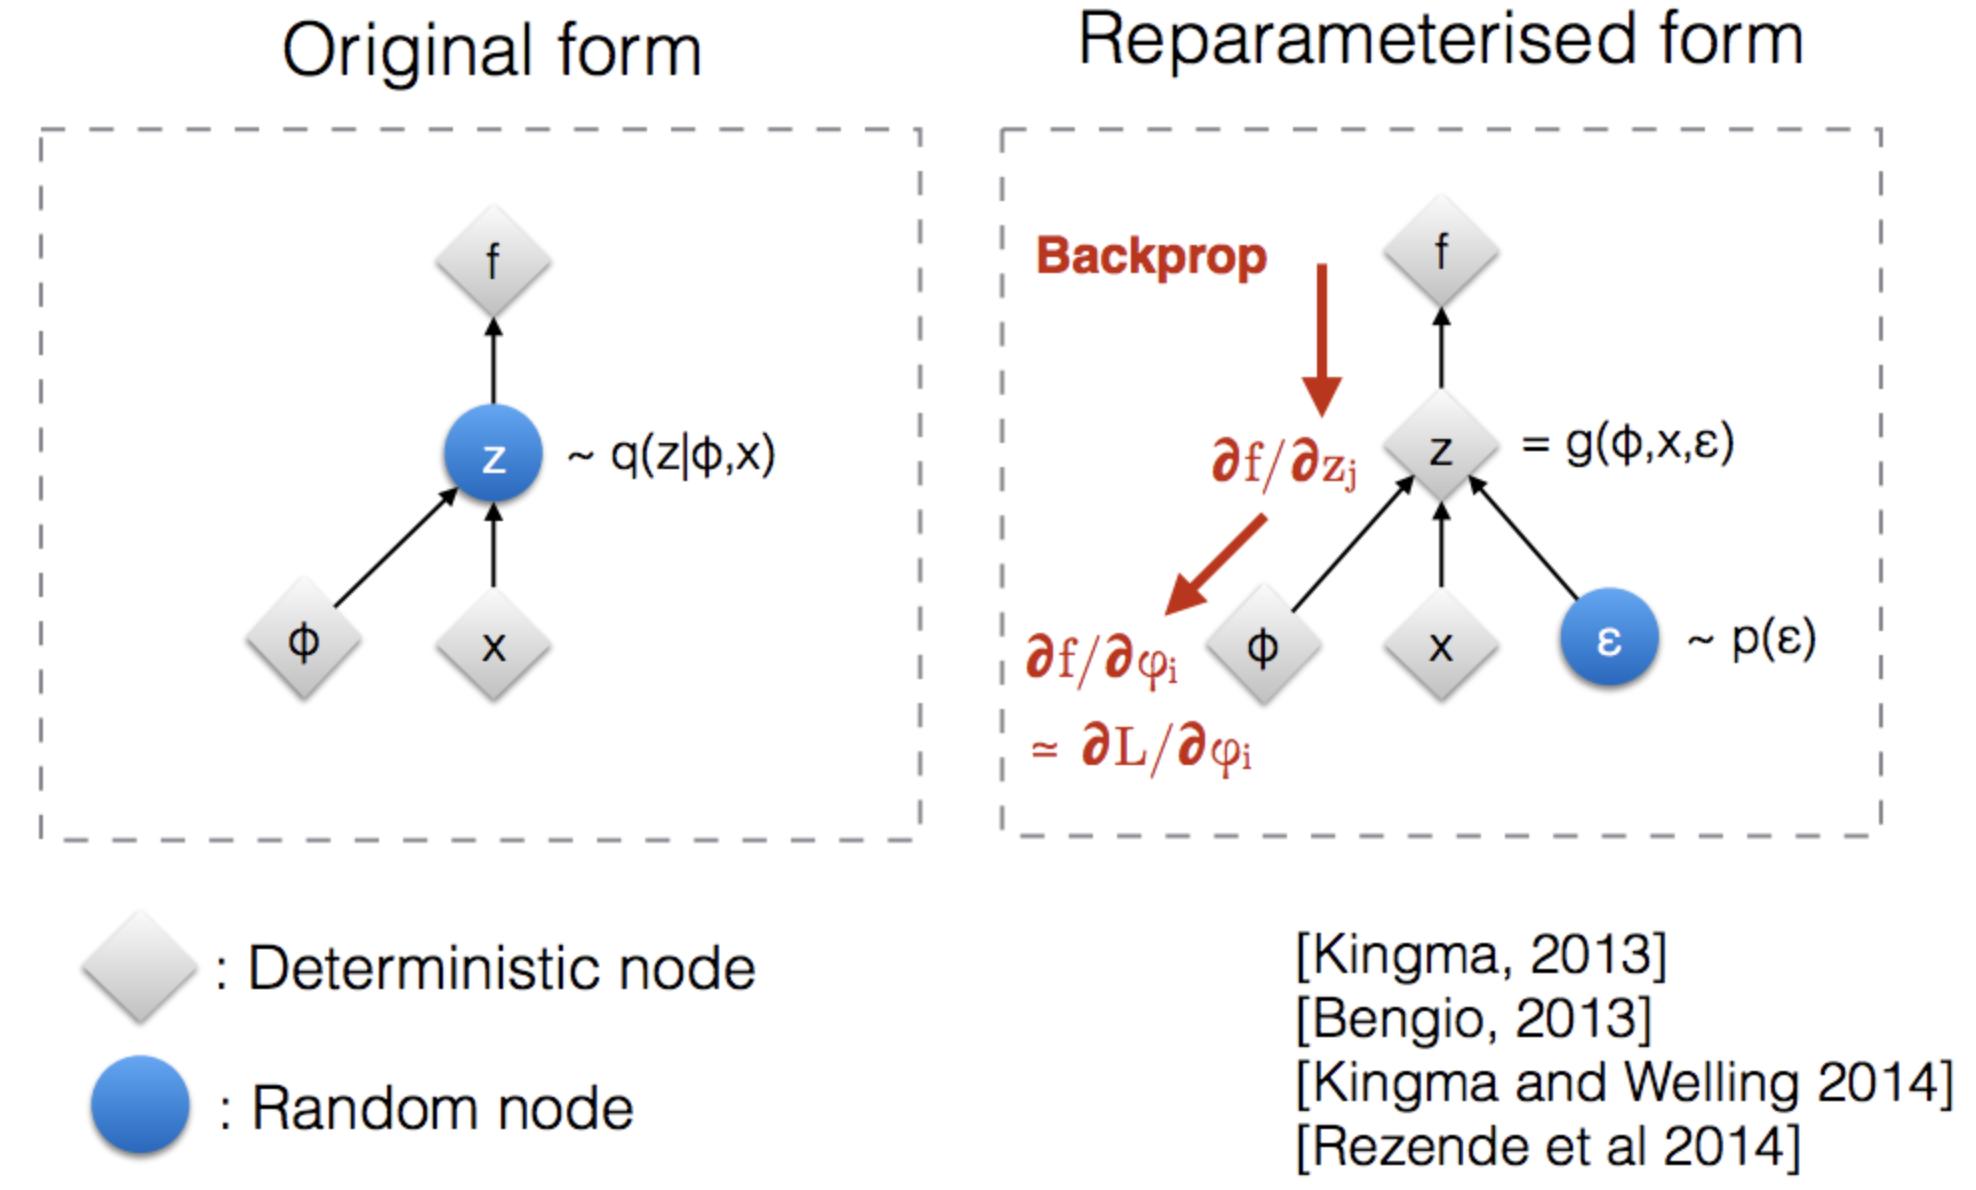
\includegraphics[width=10cm]{reparam_trick.png}
	\end{center}
\end{frame}


%-------------------------------------------------------------%

\begin{frame}
	\frametitle{VAE Models and Performance}
	
	\begin{itemize}
		\item VAEs can be used with any kind of data
		\begin{itemize}
			\item the distributions and network architecture just needs to be set accordingly
			\item e.g. it's common to use convolutions in the encoder and transpose convolutions in (Gaussian) decoder for image data
		\end{itemize}
		\item VAEs have nice learning dynamics; they tend to be easy to optimise with stable convergence
		\item VAEs have a reputation for producing blurry reconstructions of images
		\begin{itemize}
			\item Not fully understood why, but most likely related to a side effect of maximum-likelihood training
		\end{itemize}
		\item VAEs tend to only utilise a small subset of the dimensions of $\bm z$
%		\begin{itemize}
%			\item Pro: automatic latent variable selection
%			\item Con: better reconstructions should be possible given the available code-space
%		\end{itemize}
	\end{itemize}
	
\end{frame}

\begin{frame}
	\frametitle{Reconstructions Example}
	\begin{center}
		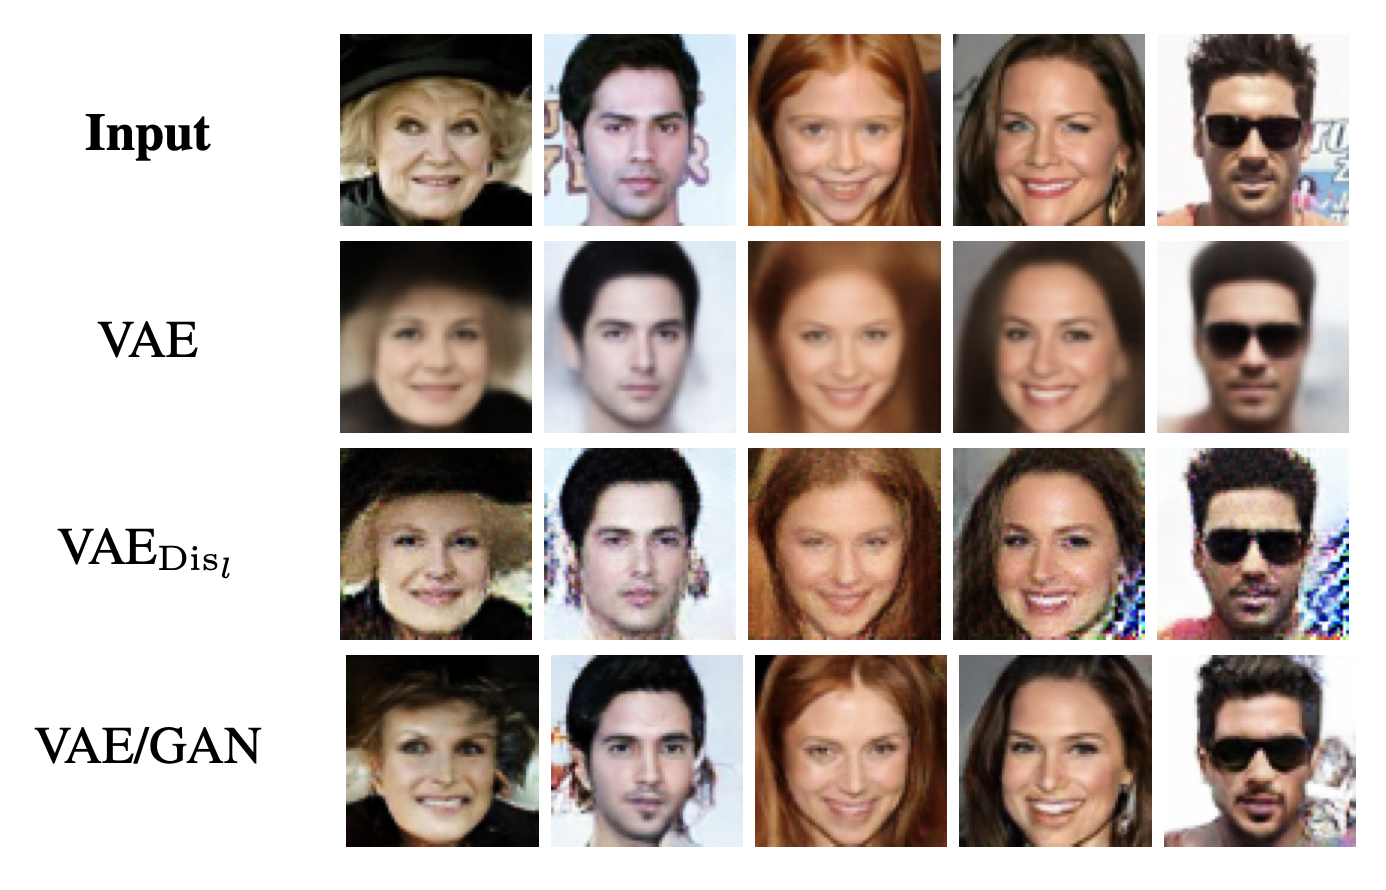
\includegraphics[width=\textwidth]{vaegan.png}
	\end{center}
\end{frame}
%-------------------------------------------------------------%
%
%\begin{frame}
%	\frametitle{Sampling Example}
%	\begin{center}
%		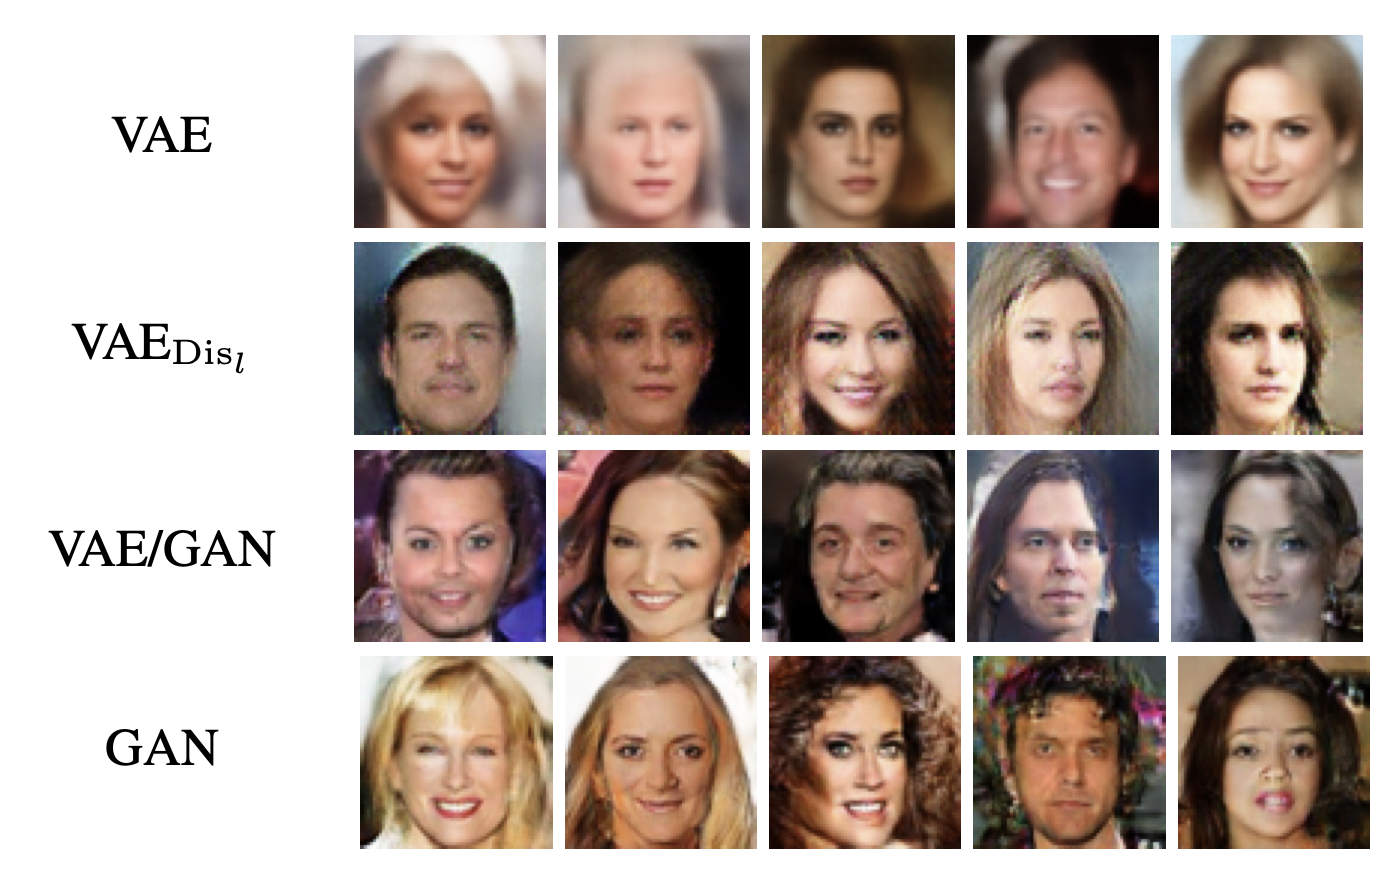
\includegraphics[width=\textwidth]{vaegan-samples.png}
%	\end{center}
%\end{frame}

\end{document}